\documentclass{article}

\usepackage[margin = 1cm]{geometry}
\usepackage{tikz}




\begin{document}

 
\begin{center}
{\Huge Human Boxplot Task}
\end{center}

\vspace{1cm}

{\huge 1. Record the height of your classmates:}

\vspace{1cm}

\begin{center}
{\large
\begin{tabular}{r|c}
\textbf{Name} & \textbf{Height (cm)} \\ \hline
JANE DOE & \\ \hline
JANE DOE & \\ \hline
JANE DOE & \\ \hline
JANE DOE & \\ \hline
JANE DOE & \\ \hline
JANE DOE & \\ \hline
JANE DOE & \\ \hline
JANE DOE & \\ \hline
JANE DOE & \\ \hline
JANE DOE & \\
\end{tabular}
}
\end{center}

\vspace{1cm}

\begin{center}
{\large
\begin{tabular}{r|c}
\textbf{Name} & \textbf{Height (cm)} \\ \hline
JOHN DOE & \\ \hline
JOHN DOE & \\ \hline
JOHN DOE & \\ \hline
JOHN DOE & \\ \hline
JOHN DOE & \\ \hline
JOHN DOE & \\ \hline
JOHN DOE & \\ \hline
JOHN DOE & \\ \hline
JOHN DOE & \\ \hline
JOHN DOE & \\ \hline
JOHN DOE & \\ \hline
JOHN DOE & \\
\end{tabular}
}
\end{center}

\pagebreak

{\huge 2. Order the heights from smallest to largest}

\vspace{0.4cm}

{\Large For the girls:}

\vspace{3cm}

{\Large and for the boys:

\vspace{3cm}

{\huge 3. Calculate a 5 number summary:}

\vspace{0.4cm}

\begin{center}
{\large
\begin{tabular}{rcrc}
\multicolumn{2}{c}{Girls} & \multicolumn{2}{c}{Boys} \\ \hline
 & & & \\
MIN: & \hspace{4cm} & MIN: & \hspace{4cm} \\ \hline
Q1:  & & Q1:  & \\ \hline
Q2:  & & Q2:  & \\ \hline
Q3:  & & Q3:  & \\ \hline
MAX: & & MAX: & \\
\end{tabular}
}
\end{center}

\vspace{0.4cm}

{\huge 2. Draw a boxplot for each.}

\vspace{0.4cm}

\begin{center}
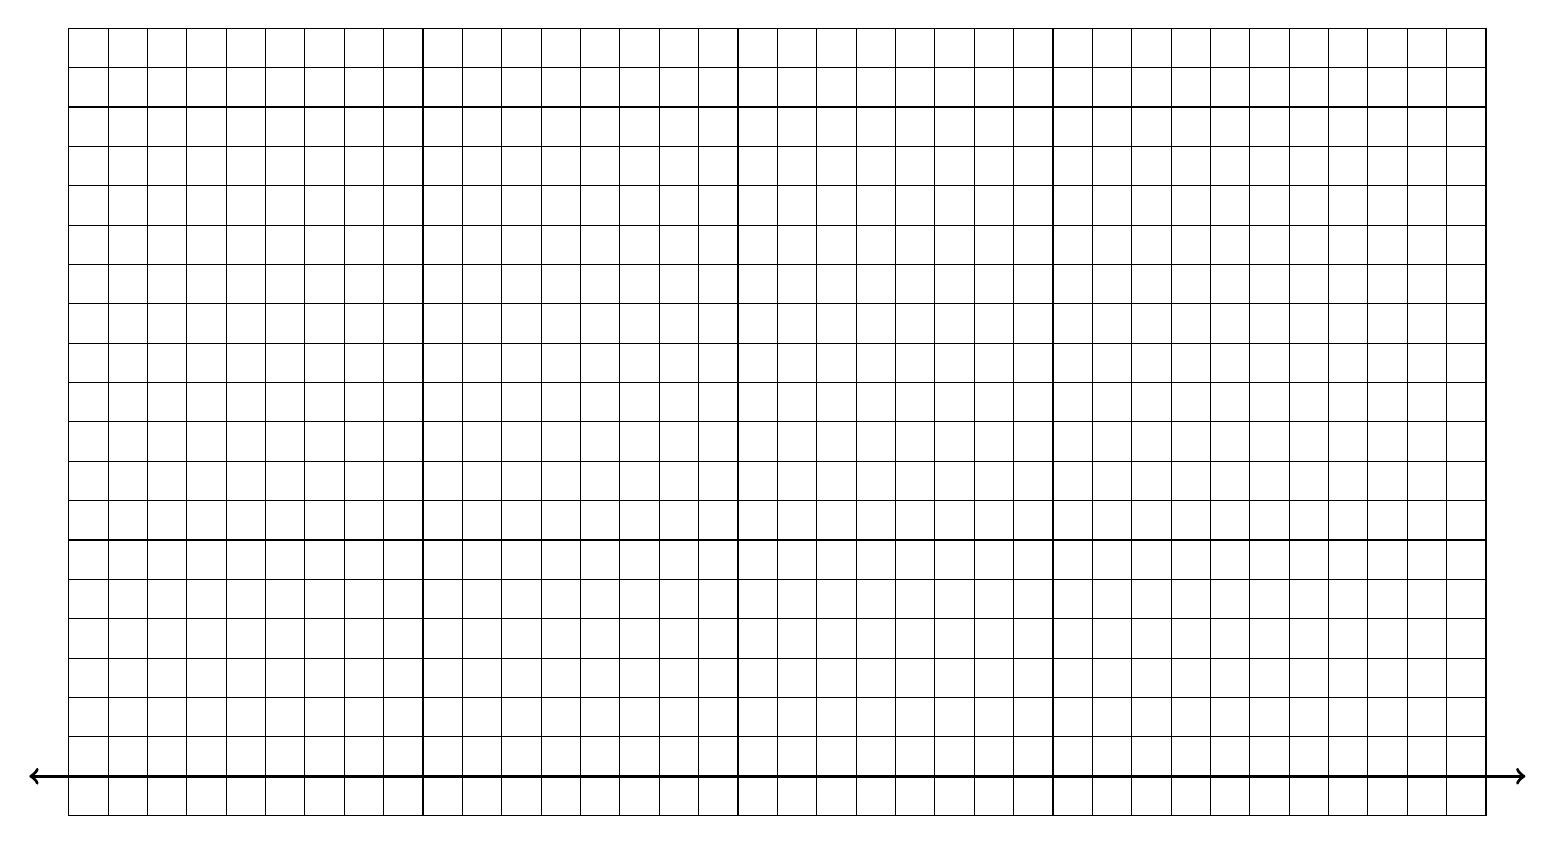
\begin{tikzpicture}
\draw[step=0.5,black,thin] (0,0) grid (18,10);
\draw[<->, very thick] (-0.5,0.5) -- (18.5, 0.5);
\end{tikzpicture}
\end{center}
\end{document}